\documentclass[../synthesis.tex]{subfiles}
\graphicspath{{\subfix{../../../../images/}}}
\begin{document}
    The \textbf{combustion method}\cite{b10}, also known as the combustion synthesis or self-sustained combustion method, is 
    a versatile and rapid technique for the synthesis of various materials, including nanophosphors. It involves 
    the exothermic reaction between fuel and oxidizer precursors, resulting in a self-sustained combustion process 
    that generates high temperatures and promotes the formation of the desired product. 
    The combustion method offers several advantages, including simplicity, rapid synthesis, and the ability to 
    produce nanophosphors with fine particle sizes and high purity. The high temperatures generated during the 
    combustion process promote the formation of crystalline nanophosphors with controlled properties. However, 
    careful control of the stoichiometry and reaction conditions is crucial to ensure reproducibility and obtain 
    the desired product.Here is an overview of the combustion method:
    \begin{Figure}
        \centering
        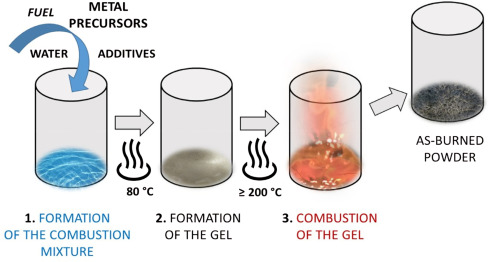
\includegraphics[width=0.8\linewidth]{combustion.jpg}
        \captionof{figure}{Synthesis using Combustion Method\cite{a10}}\label{fig:combustion}
    \end{Figure}
    \begin{itemize}
        \item \textbf{Selection of Precursor Materials: } Choose appropriate precursor materials that contain the 
        necessary elements for the composition of the nanophosphor. These precursors typically include a fuel and 
        an oxidizer.
        \item \textbf{Weighing and Mixing: }Accurately weigh and thoroughly mix the fuel and oxidizer precursors 
        in the desired stoichiometric ratio. The mixing process is crucial to ensure a homogenous distribution of 
        the reactants and promote a complete reaction.
        \item \textbf{Pelletization or Pressing: }Depending on the application and desired final form of the 
        nanophosphor, the mixture of precursor powders may be pressed into pellets or compacted using a hydraulic 
        press to obtain a solid compact.
        \item \textbf{Ignition: }Apply an external ignition source, such as a spark or a flame, to initiate the 
        combustion reaction. The exothermic reaction between the fuel and oxidizer precursors releases a 
        significant amount of heat, leading to self-sustained combustion.
        \item \textbf{Combustion Reaction: }The combustion reaction generates high temperatures, often exceeding 
        $1000^{\circ}C$, which facilitates rapid reaction kinetics and the formation of the desired nanophosphor. 
        The reaction is typically completed within seconds to minutes.
        \item \textbf{Cooling and Grinding: }After the combustion reaction is complete, the sample is allowed to 
        cool to room temperature. The resulting product is typically in the form of a porous solid or powder. 
        Grinding or milling can be performed to break up any agglomerates and obtain a fine powder of the 
        nanophosphor.
    \end{itemize}
\end{document}

